\documentclass[11pt]{article}
\usepackage[a4paper,margin=18mm]{geometry}
\usepackage{fontspec}
\setmainfont{Latin Modern Roman}
\usepackage{amsmath,amssymb,amsthm,amscd,graphicx,color}
\usepackage{xurl}
\usepackage[unicode,hidelinks]{hyperref}
\allowdisplaybreaks
\setlength\emergencystretch{3em}

\makeatletter
\newtheorem{theorem}{Theorem}
\newtheorem*{theorem*}{Theorem}
\newtheorem{lemma}{Lemma}
\newtheorem*{lemma*}{Lemma}
\newtheorem{corollary}{Corollary}
\newtheorem*{corollary*}{Corollary}
\newtheorem{proposition}{Proposition}
\newtheorem*{proposition*}{Proposition}
\newtheorem{conjecture}{Conjecture}
\newtheorem*{conjecture*}{Conjecture}
{\theoremstyle{definition} \newtheorem{definition}{Definition}
\newtheorem*{definition*}{Definition}
\newtheorem{example}{Example}
\newtheorem*{example*}{Example}
\newtheorem{remark}{Remark}
\newtheorem*{remark*}{Remark}
\newtheorem{note}{Note}
\newtheorem*{note*}{Note}
}

\makeatother



\begin{document}
\begin{center}\Large A complex analytic monic cubic 3-web germ with distinct generic directions, unequal-weight linear symmetry, identically zero normalized Chern connection and the specified commuting lifted idempotents reconstructs a Frobenius 3-fold germ with isotropic unity\end{center}
\noindent\textbf{Stable ID:} 2185\par
\noindent\textbf{Authors:} Sergey I. Agafonov\par
\noindent\textbf{Original work:} Frobenius 3-Folds via Singular Flat 3-Webs\par
\noindent\textbf{Version:} Official SIGMA 8 (2012) article 078, DOI 10.3842/SIGMA.2012.078; journal PDF and native TeX acquired 2026-10-01, exact bytes pinned by SHA256\par
\noindent\textbf{Selected task scope:} Full Theorem2 under the complex-analytic germ setup: the monic cubic ODE p\textasciicircum{}3+\allowbreak{}S(x,y)p\textasciicircum{}2+\allowbreak{}A(x,y)p+\allowbreak{}B(x,y)=\allowbreak{}0 defines a 3-web with pairwise distinct directions generically. It admits X=\allowbreak{}w\_x x partial\_x+\allowbreak{}w\_y y partial\_y with w\_x!=\allowbreak{}w\_y; the Chern connection form gamma of normalization(5) is identically0. With K=\allowbreak{}-1, take v\_i and alpha,beta exactly as(10), and lifted e1=\allowbreak{}alpha partial\_t+\allowbreak{}v1,e2=\allowbreak{}beta partial\_t+\allowbreak{}v2 as(7); require[e1,e2]=\allowbreak{}0. Then a Frobenius3-fold germ with<e,e>=\allowbreak{}0 has that booklet web. The author takes metric(3) with delta1, unity partial\_t and Euler E=\allowbreak{}(2w\_y-w\_x)t partial\_t+\allowbreak{}X. This does not claim that closed/holomorphic Chern form and a symmetry alone imply the conclusion.\par
\noindent\textbf{Difficulty:} H2: The proof reconstructs an invariant metric and multiplication from multivalued web-root fields, then turns their commutativity and normalized connection equations into a compatible system for an analytic associativity potential. The weight matching and potential reconstruction produce holomorphic Frobenius tensors through the singular web point, a nonlinear geometric inverse construction beyond ordinary qualification differential geometry.\par
\noindent\textbf{Editorial boundary note (not author text):} The full original Theorem2 is retained with the analytic Frobenius/booklet definitions, metric weight analysis, normalized cubic-root Chern form, full lifted idempotents and their orthogonality/commutativity equations, hydrodynamic system and complete Lemma1 potential reconstruction. Gamma must vanish identically in the stated normalization and the displayed first two lifted fields must commute. The source idempotent-label notice is retained. Named Dubrovin/associativity and earlier booklet-web results remain cited prerequisites; nonisotropic and normal-form classifications are not selected.\par
\noindent\textbf{Source:} \url{https://sigma-journal.com/2012/078/}\quad DOI: \url{https://doi.org/10.3842/SIGMA.2012.078}\par
\noindent\textbf{License and attribution:} Copyright retained by the named authors. Published by SIGMA under CC BY 4.0: \url{https://creativecommons.org/licenses/by/4.0/}. Source: \url{https://sigma-journal.com/about.html}. Adaptation consists of standalone excerpt formatting, cover and numbering restoration; original author language and mathematical text are retained.\par
\noindent\textbf{Editorial symbol notice (not author text):} Source annotation only: equation(7) repeats the label e1 on its third displayed idempotent. The preceding sum-to-unity statement(1), the explicit coefficient(1-alpha-beta), and the subsequent orthogonality equations identify that third vector as the e3 used in the construction. Source labels/formulas remain unchanged; the selected assumptions use the separately unambiguous first two lifted fields.\par
\medskip\hrule\medskip\noindent\textbf{Author text begins below.}\par
\setcounter{section}{0}
\setcounter{subsection}{0}
\setcounter{subsubsection}{0}
\setcounter{equation}{0}
% Original source lines 56--113
\section{Introduction}

The theory of Frobenius manifolds, having its origin in theoretical physics, has deep interrelations with apparently very dif\/ferent areas of mathematics: Gromov--Witten invariants and quantum cohomology, integrable systems, singularity, deformation of f\/lat connections etc.
We discuss a~new aspect of this fruitful and fast developing theory: its relations with the classical chapter of dif\/ferential geometry, namely the web theory.

The notion of Frobenius manifold, introduced by B.~Dubrovin (see~\cite{Df} and~\cite{Mf}), is a geometric translation of the theory of WDVV-equations that arise originally in the physical context of two-dimensional topological f\/ield theory.
\begin{definition}\label{defFrob}
A Frobenius manifold is a complex analytic manifold $M$ equipped with the following
analytic objects:
\begin{enumerate}\itemsep=0pt
\item[1)] a commutative and associative multiplication on $T_pM$,
\item[2)] an invariant non-degenerate f\/lat inner product: $\langle u \cdot v, w \rangle = \langle u, v \cdot w \rangle $,
\item[3)] a constant unity vector f\/ield $e$: $\nabla e=0$, $e \cdot v=v$ $\forall\, v\in TM$,
\item[4)] a linear Euler vector f\/ield $E$: $\nabla (\nabla E)=0$,
\end{enumerate}
satisfying the following conditions:
\begin{itemize}\itemsep=0pt
\item the f\/low of $E$ re-scales the
multiplication and the inner product,
\item 4-tensor $(\nabla_z c)(u,v,w)$ is symmetric in
$u$, $v$, $w$, $z$, where
\[
c(u,v,w):=\langle u\cdot v,w\rangle.
\]
\end{itemize}
In this def\/inition, the symbol $\nabla$ stands for the Levi-Civita connection of the inner product $\langle\ ,\ \rangle$.
\end{definition}
The following geometric construction of $3$-web via Frobenius $3$-fold was proposed in~\cite{Aw}.
Consider a {\it massive} Frobenius $3$-fold $M$, which means that the algebra $T_pM$ is semi-simple for each $p\in U$ for some open set $U\subset M$. Then $T_pM$ is the direct
product of one-dimensional algebras spanned by idempotents
\begin{equation}\label{mult}
T_pM=\mathbb C \{e_1\}\otimes \mathbb C \{e_2\}\otimes \mathbb C\{e_3\}, \qquad e_i\cdot e_j=\delta_{ij}e_i.
\end{equation}
In this setting, the unity vector f\/ield is
\[
e=e_1+e_2+e_3.
\]
Let $S$ be a surface transverse to the unit vector f\/ield $e$, then 3
planes spanned by $\{e,e_i\}$ cut 3 directions on $T_pS$ (see Fig.~\ref{booklet} on the left).
The integral curves of these direction f\/ields build a {\it flat} (or {\it hexagonal}) {\it $3$-web}, i.e., at the points with pairwise distinct web directions, this web is locally biholomorphic to 3 families of parallel lines in the plane.
Due to the existence of {\it canonical Dubrovin} coordinates (see~\cite{Di}), the distributions $\{e,e_i\}$ are integrable, integral surfaces of each of the distributions being formed by the integral curves of the unity vector f\/ield~$e$. Thus for each point in $M$ there are 3 integral surfaces intersecting along such a curve. These surfaces cut $S$ along the constructed web. This justif\/ies the following def\/inition (see also Fig.~\ref{booklet} on the right).
\begin{figure}[th]\centering
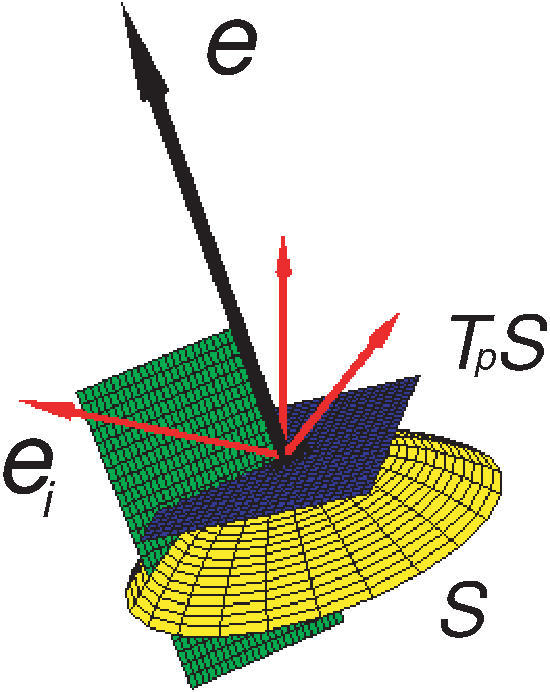
\includegraphics[width=40mm]{../assets/2185/Agafonov-Fig1a.pdf} \qquad\quad
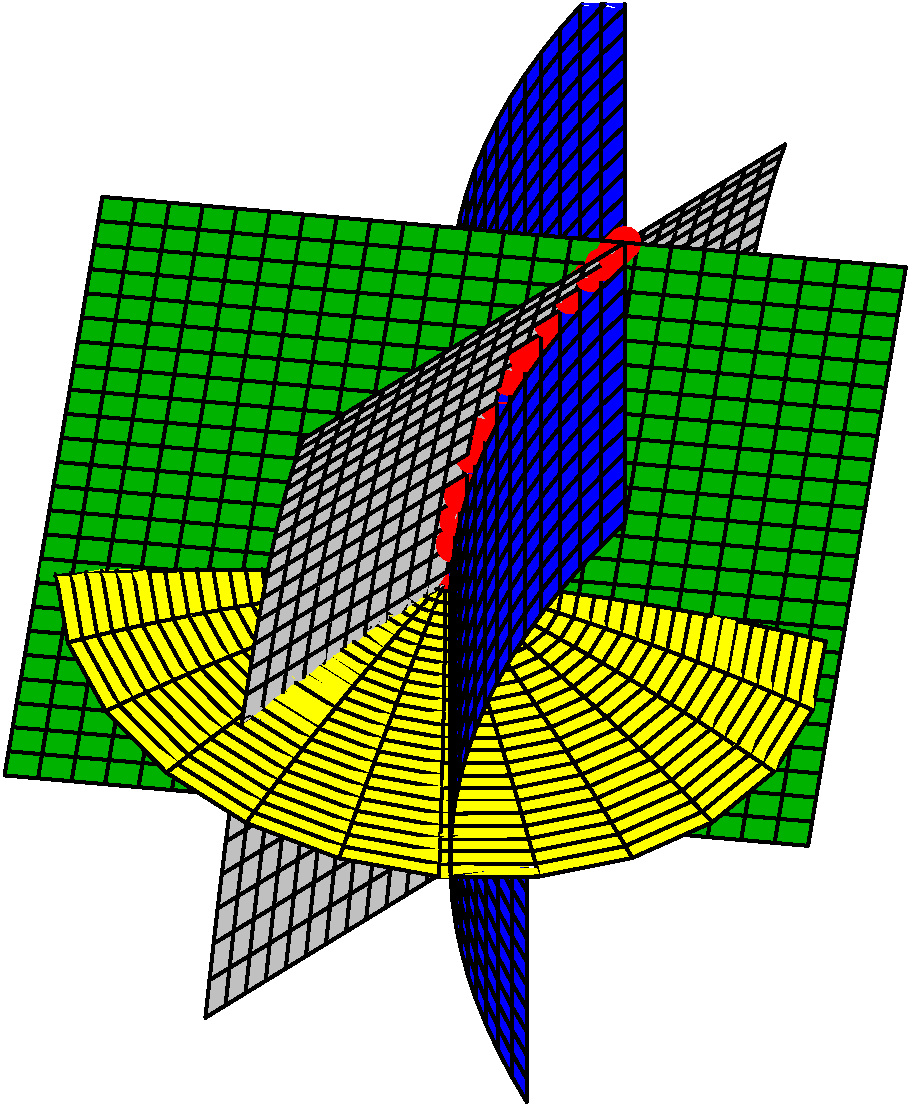
\includegraphics[width=40mm]{../assets/2185/Agafonov-Fig1b.pdf}
%\includegraphics[width=80mm]{aaa}
%\hspace{-0.5cm} \epsfig{file=idgif_eps.eps,width=80mm}
%\qquad \put(1,8){ \epsfig{file=booklet.eps,width=40mm}}
\caption{Construction of a booklet $3$-webs from Frobenius $3$-folds.}
%$e_i$ \quad $T_p S$ \quad $S$ \quad $e$
\label{booklet}
\end{figure}

\begin{definition}
The constructed web is called a booklet $3$-web.
\end{definition}
The web directions of a booklet $3$-web are well-def\/ined everywhere (see~\cite{Aw}), maybe with multiplicity.
We call a point {\it regular or non-singular} if the web directions at this point are pairwise distinct. The locus of singular points is called the discriminant curve.
By def\/inition, a hexagonal $3$-web does not have any local invariants at regular points. Its ``personality'' is encoded in the behavior at \emph{singular points}, where at least 2 web directions coincide.
\setcounter{section}{1}
\setcounter{subsection}{0}
\setcounter{subsubsection}{0}
\setcounter{equation}{2}
% Original source lines 155--170
Consider the map $\pi_e: M\to S$ that assigns to each $p\in M$ the intersection
of its trajectory under the f\/low of $e$ with $S$.
Then the vector f\/ields $e_i$ and $v_i:=d\pi_e(e_i(p))$ are $\pi$-related: $d\pi_e(e_i(p))=v_i(\pi_e(p))$.
Therefore $[v_i,v_j]=0$.

If we have a f\/lat $3$-web, then the natural candidates for $v_i$ are the commuting web direction vector f\/ields. We recover idempotents in the form $e_i=v_i+\alpha_i\partial_t$, where $t$ is a third local coordinate on a Frobenius $3$-fold germ to be constructed.
The functions $\alpha_i$ are subjected to the following conditions:
\begin{enumerate}\itemsep=0pt
\item[1)] $\sum e_i=\partial_t,$
\item[2)] $e_i$ commute: $[e_i,e_j]=0$,
\item[3)] there is a non-degenerate f\/lat metric $g$ with $g(e_i,e_j)=0$, $i\ne j$,
\item[4)] the f\/low of $X+w_3t\partial_t$ re-scales the metric for a suitable weight $w_3$.
\end{enumerate}
(By metric we understand a non-degenerate inner product.)
It turns out that these conditions can be satisf\/ied, the analyticity of the Chern connection form being crucial for the existence of the metric $g$.
We def\/ine the multiplication by formula~(\ref{mult}). The obtained structure is that of Frobenius $3$-fold since the above conditions on $\alpha_i$ are equivalent to the associativity equation with dilatation symmetry.
\setcounter{section}{2}
\setcounter{subsection}{0}
\setcounter{subsubsection}{0}
\setcounter{equation}{2}
% Original source lines 249--285
\section{Metric in f\/lat coordinates}
In this section we present forms of invariant metrics for our Frobenius $3$-folds in f\/lat coordinates.
For the case when all the weights of the Euler vector f\/ields are distinct,
they were obtained for arbitrary~$n=3$ in~\cite{Df}.
Here we consider a bit weaker hypothesis that the weights of~$x$ and~$y$ are not equal.
We are looking for a constant matrix
\[g=
\begin{pmatrix}
g_{tt}&g_{tx}&g_{ty}\\
g_{tx}&g_{xx}&g_{xy}\\
g_{ty}&g_{xy}&g_{yy}
\end{pmatrix},
\]
where $g_{tt}=\langle e$, $e\rangle=\langle\partial_t,\partial_t\rangle$,
$g_{tx}=\langle\partial_t,\partial_x\rangle $, \dots, $g_{yy}=\langle\partial_y,\partial_y\rangle $, satisfying
$L_E(g)={\rm const}\cdot g$. (The local f\/low $\exp(Ea)$ re-scales the metric.)
One has $L_E(g)_{tt}=-2w_tg_{tt}$, $L_E(g)_{tx}=(-w_t-w_x)g_{tx}$, \dots, $L_E(g)_{yy}=-2w_yg_{yy}$.
Therefore the non-vanishing entries in $g$ must be of the same weight.
Observe also that for each $3$-web in the classif\/ication list the inequality $w_x\ne w_y$ holds true.

$\bullet$ {\it Metric with $\langle e,e\rangle=0$.}
As $w_{tx}\ne w_{ty}$ and the metric $g$ is non-degenerate exactly one of the the entries $g_{tx}$, $g_{ty}$
is non-vanishing. Suppose that $g_{ty}=1$. Now $g_{xx}\ne 0$ since $g$ is non-degenerate.
This implies $g_{xy}=0$, $g_{yy}=0$ and $2w_x=w_t+w_y$.
If $g_{ty}=0$ then, similarly, one normalizes $g_{tx}=1$ and obtains $g_{yy}\ne 0$, $g_{xx}=g_{xy}=0$.

Suppose $g_{xx}=\delta\ne 0$ then $\langle e_1,e_2\rangle =\langle e_1,e_3\rangle =0$ implies that the weights of $p_i$ are zero. This is not possible for our singular webs. Therefore $g_{xx}$ must vanish and the form of the matrix $g$ is
\begin{equation}\label{metric0}
g=
\begin{pmatrix}
0 & 1 & 0\\
1 & 0 & 0\\
0 & 0 & \delta
\end{pmatrix},
\end{equation}
where $\delta \ne 0$.

\setcounter{section}{3}
\setcounter{subsection}{0}
\setcounter{subsubsection}{0}
\setcounter{equation}{3}
\setcounter{theorem}{1}
% Original source lines 303--448
\section{Idempotents}
In this section we determine idempotents $e_i$ using the following 2 facts:
\begin{enumerate}\itemsep=0pt
\item[1)] the metric, being invariant, is diagonal in the basis $\{e_1,e_2,e_3\}$,
\item[2)] the idempotents commute.
\end{enumerate}
Suppose that the following implicit cubic ODE def\/ines our $3$-web:
\begin{equation}\label{flat_cub}
p^3+S(x,y)p^2+A(x,y)p+B(x,y)=0.
\end{equation}
Let $p_1$, $p_2$, $p_3$ be the roots of~(\ref{flat_cub}) at a point
$(x,y)$ outside the discriminant curve. The following 1-forms vanish on the
solutions
\begin{gather}
\sigma_1=(p_2-p_3)(dy-p_1dx),\nonumber\\
\sigma_2=(p_3-p_1)(dy-p_2dx),\nonumber\\
\sigma_3=(p_1-p_2)(dy-p_3dx)\label{normalized forms}
\end{gather}
and satisfy
\[
\sigma_1+\sigma_2 + \sigma_3=0.
\]
Let us introduce an ``area'' form by
\[
\Omega =\sigma_1\wedge
\sigma_2=\sigma_2\wedge \sigma_3=\sigma_3\wedge
\sigma_1=(p_1-p_2)(p_2-p_3)(p_3-p_1)dy\wedge dx.
\]
 The Chern
connection form is def\/ined as (see~\cite{Be})
\[
\gamma:
=h_2\sigma_1-h_1\sigma_2=h_3\sigma_2-h_2\sigma_3=h_1\sigma_3-h_3\sigma_1,
\]
where $h_i$ verify the relations
\[
d\sigma_i=h_i\Omega.
\]
The web is f\/lat if\/f the connection form
is closed: $d(\gamma)=0$. This implies $d\sigma_i=\gamma \wedge \sigma_i$ and gives an integrating factor $k$ of the forms $\sigma_i$ as a solution to the following equation
\begin{gather*}%\label{dk}
dk=-\gamma k.
\end{gather*}
Computing the Chern connection form in terms of roots $p_i$ and using the Viete formulas one gets
\[
\gamma =\frac{\gamma_1dx+\gamma_2dy}{-D},
\]
where
\begin{gather*}
\gamma_1=\big(4BS^2-3AB-SA^2\big)S_x+B(SA-9B)S_y+(2A^2-6SB)A_x\nonumber\\
\hphantom{\gamma_1=}{}
+2B(3A-S^2)A_y+(9B-SA)B_x+\big(AS^2-4A^2+3SB\big)B_y,\nonumber\\
\gamma_2=\big(6SB-2A^2\big)S_x-2B\big(3A-S^2\big)S_y+(SA-9B)A_x\nonumber\\
\hphantom{\gamma_2=}{}
 + \big(4A^2-AS^2-3SB\big)A_y+\big(6A-2S^2\big)B_x+\big(2S^3+18B-8SA\big)B_y,%\label{connectionSAB}
\end{gather*}
and $D$ is the discriminant of~(\ref{flat_cub}) with respect to $p$
\[
D=18SAB+S^2A^2-4A^3-27B^2-4BS^3.
\]
We also need to know how the connection form in the normalization~(\ref{normalized forms})
is transformed when we change the local coordinates
\[
\bar{y}=f(x,y), \qquad \bar{x}=g(x,y).
\]
One f\/inds without dif\/f\/iculty that the forms $\bar{\sigma_i}$
in the new coordinates are related to the forms in old ones by
\begin{gather*}%\label{form transform}
\bar{\sigma_i}=\frac{(f_yg_x-f_xg_y)^2\sigma_i}{g_x^3-Sg_x^2g_y+Ag_xg_y^2-Bg_y^3}.
\end{gather*}
Therefore (see~\cite{Be})
\begin{equation}\label{connection transforms}
\bar{\gamma}=\gamma+d\ln\left(\frac{(f_yg_x-f_xg_y)^2}{g_x^3-Sg_x^2g_y+Ag_xg_y^2-Bg_y^3}\right).
\end{equation}
Let $v_i=\xi_i \partial_x+\eta_i\partial_y$ be commuting multi-valued vector f\/ields,
whose trajectories are the web leaves. They may have singularities at singular points:
with $K$ satisfying $\frac{dK}{K}=\gamma $ we have
\begin{gather*}%\label{v0}
v_1=\frac{K(\partial_x +p_1 \partial_y)}{(p_3-p_1)(p_1-p_2)},\qquad
v_2=\frac{K(\partial_x +p_2 \partial_y)}{(p_1-p_2)(p_2-p_3)},\qquad
v_3=\frac{K(\partial_x +p_3 \partial_y)}{(p_2-p_3)(p_3-p_1)}.
\end{gather*}
Here $x$, $y$ are restrictions on $S$ of f\/lat coordinates in $M$, in which the Euler vector f\/ield has the form $E=w_tt\partial_t+w_xx\partial_x+w_yy\partial_y$. A subtle point is that f\/lat coordinates are not necessarily the coordinates used for the normal forms: they are related to them by some coordinate transform preserving $X$.

The idempotents are
\begin{equation}\label{idempotents}
e_1=\alpha \partial_t+v_1, \qquad e_2=\beta \partial_t+v_2,\qquad e_1=(1-\alpha -\beta) \partial_t+v_3,
\end{equation}
where the components $\alpha$, $\beta$ are to be def\/ined by the orthogonality condition
\begin{equation}\label{orthogonal}
\langle e_1,e_2\rangle =\langle e_2,e_3\rangle =\langle e_3,e_1\rangle =0.
\end{equation}

$\bullet$ {\it Metric with $\langle e,e\rangle =0$.}
Equations~(\ref{orthogonal}) give
\begin{equation}\label{dfor0}
\delta=-1/K.
\end{equation} Adjusting the integration constant so that $K=-1$ we have $\delta =1$ and
\begin{equation}\label{alphabeta0}
\alpha =\frac{p_2p_3-p_1(p_2+p_3)}{2(p_1-p_2)(p_1-p_3)},\qquad \beta =\frac{p_1p_3-p_2(p_1+p_3)}{2(p_2-p_1)(p_2-p_3)}.
\end{equation}
Since $dK=0$, we see that $\gamma_1=\gamma_2=0$.
The equation $[e_1,e_2]=0$ reads as $v_1(\beta)=v_2(\alpha)$ and obviously implies $[e_1,e_3]=[e_2,e_3]=0$.
The above 3 equations $\gamma_1=\gamma_2=v_1(\beta)-v_2(\alpha)=0$
can be resolved with respect to $S_x$, $A_x$, $B_x$
to give the following system of hydrodynamic type
\begin{gather}\label{WDVV0}
S_x= \frac{1}{2}A_y,\qquad
A_x= 2By,\qquad
B_x= SB_y+BS_y-\frac{1}{2}AA_y.
\end{gather}
\begin{lemma}\label{web_ass_0}
Suppose that the solution web of ODE~\eqref{flat_cub} satisfies the following conditions:
\begin{enumerate}\itemsep=0pt
\item[$1)$] it admits an infinitesimal symmetry $X=w_xx\partial_x+w_yy\partial_y$ with $w_x\ne w_y$,
\item[$2)$] the coefficients $S$, $A$, $B$ satisfy the system of PDEs~\eqref{WDVV0}.
\end{enumerate}
Then there is a Frobenius $3$-fold germ with $\langle e,e\rangle =0$ whose booklet web is the solution web of~\eqref{flat_cub}.
\end{lemma}
\begin{proof}
Equations~(\ref{WDVV0}) ensures the local existence of a function $f(x,y)$ satisfying
$f_{yyy}=S$, $f_{yyx}=\frac{1}{2}A$, $f_{yxx}=B$, $f_{xxx}=BS-\frac{1}{4}A^2$.
Thus we obtain the associativity equation
\begin{equation}\label{assPoly}
f_{xxx}=f_{yyy}f_{yxx}-f^2_{yyx}.
\end{equation}
(See~\cite{MFa} where the equivalence of~(\ref{WDVV0}) and~(\ref{assPoly}) was established and~\cite{Al} where equations of these types were studied.)
Since the web admits an inf\/initesimal symmetry $X$, the function~$f$ is weighted homogeneous and def\/ines a germ of Frobenius $3$-fold with $\langle e,e\rangle =0$ (see~\cite{Df}). Equation~(\ref{flat_cub}) def\/ines the corresponding characteristic web of the above associativity equation. Hence the web is the booklet web of the constructed Frobenius $3$-fold germ (see~\cite{Aw}).
\end{proof}
The value of the lemma is that it makes unnecessary the checking the potentiality condition for the 4-tensor $(\nabla_z c)(u,v,w)$ in Def\/inition~\ref{defFrob}.
\begin{theorem}\label{web_Frobenius_0}
Suppose that the solution web of ODE~\eqref{flat_cub} satisfies the following conditions:
\begin{enumerate}\itemsep=0pt
\item[$1)$] it admits an infinitesimal symmetry $X=w_xx\partial_x+w_yy\partial_y$ with $w_x\ne w_y$,
\item[$2)$] its Chern connection form vanishes identically $\gamma=0$,
\item[$3)$] the vector fields $e_1$, $e_2$ commute, where $\alpha$, $\beta$ are as in~\eqref{alphabeta0}.
\end{enumerate}
Then there is a Frobenius $3$-fold germ with $\langle e,e\rangle=0$
whose booklet web is the solution web of~\eqref{flat_cub}.
\end{theorem}
\begin{proof}
Def\/ine a metric by~(\ref{metric0}) with $\delta=1$,
the multiplication as the direct sum of one-dimensional algebras with unities~(\ref{idempotents}),
and the Euler vector f\/ield by $E=w_tt\partial_t+X$ with $w_t=2w_y-w_x$.
Then Lemma~\ref{web_ass_0} ensures that the def\/ined structure is that of Frobenius \mbox{$3$-fold}.
\end{proof}
\begin{thebibliography}{99}
\bibitem[1]{Aw}
Agafonov S.I., Flat 3-webs via semi-simple {F}robenius 3-manifolds,
  \href{http://dx.doi.org/10.1016/j.geomphys.2011.10.020}{\textit{J.~Geom. Phys.}} \textbf{62} (2012), 361--367, \href{http://arxiv.org/abs/1108.1997}{arXiv:1108.1997}.

\bibitem[2]{Al}
Agafonov S.I., Linearly degenerate reducible systems of hydrodynamic type,
  \href{http://dx.doi.org/10.1006/jmaa.1996.5357}{\textit{J.~Math. Anal. Appl.}} \textbf{222} (1998), 15--37.

\bibitem[6]{Be}
Blaschke W., Einf\"uhrung in die {G}eometrie der {W}aben, Birkh\"auser Verlag,
  Basel und Stuttgart, 1955.

\bibitem[8]{Df}
Dubrovin B., Geometry of {$2$}{D} topological f\/ield theories, in Integrable
  Systems and Quantum Groups ({M}ontecatini {T}erme, 1993), \href{http://dx.doi.org/10.1007/BFb0094793}{\textit{Lecture
  Notes in Math.}}, Vol.~1620, Springer, Berlin, 1996, 120--348,
  \href{http://arxiv.org/abs/hep-th/9407018}{hep-th/9407018}.

\bibitem[9]{Di}
Dubrovin B., Integrable systems in topological f\/ield theory, \href{http://dx.doi.org/10.1016/0550-3213(92)90137-Z}{\textit{Nuclear
  Phys.~B}} \textbf{379} (1992), 627--689.

\bibitem[12]{Mf}
Manin Yu.I., Frobenius manifolds, quantum cohomology, and moduli spaces,
  \textit{American Mathematical Society Colloquium Publications}, Vol.~47,
  American Mathematical Society, Providence, RI, 1999.

\bibitem[13]{MFa}
Mokhov O.I., Ferapontov E.V., Associativity equations of two-dimensional
  topological f\/ield theory as integrable {H}amiltonian nondiagonalizable
  systems of hydrodynamic type, \href{http://dx.doi.org/10.1007/BF02509506}{\textit{Funct. Anal. Appl.}} \textbf{30} (1996),
  195–--203, \href{http://arxiv.org/abs/hep-th/9505180}{hep-th/9505180}.

\end{thebibliography}
\end{document}
